\newgeometry{textwidth=16cm}
\chapter[Corrections à la dispersion]{Corrections à la Dispersion}
\minitoc
\restoregeometry

\newpage

	\section*{Introduction}
\spacing{1.5}
	
	En mécanique quantique les molécules sont décryptes comme un assemblage de noyaux et d'électrons attaché aux effets classiques et quantiques. Même en considérant les noyaux comme fixes, le comportement des électrons constituent un problème complique à N corps. Pour la résolution de l'équation de Schrödinger la théorie de la fonctionnelle de la densité établie une alternative intéressante pour aborder ce problème, grâce à la description du système par sa densité électronique\cite{adamo2014decrire}.
	
	\bigskip
	La DFT a eu un grand succès dans l'étude de systèmes dans lesquels la taille fait impossible un calcul ab initio Post Hartree- Fock, pour la compréhension parmi différents sujets en sciences et technologie.\cite{neese2009prediction,sanchez1997density,waller2006hybrid}
	\bigskip
	
	Cependant cette méthode présente déficiences au moment de traduire la dispersion dans les systèmes et les interactions du van der Waals, voire le théorème Hohenberg- Kohn prédit que si nous connaissons la fonctionnelle correcte, nous pourrions obtenir l’énergie à l’état fondamental en arrivant à son point minimum, donc la difficulté provient des fonctionnelles approximatifs. Local et semi local fonctionnelles  ne peuvent pas reproduire le comportement asymptotique de $1/R^{6}$, comme cela affecte les molécules où il y a une considérable superposition de la densité est inconnue. Il existe une corrélation claire de l'incapacité de décrire les interactions de Van der Waals avec la fonctionnelle d'échange GGA dans la région de faible densité et gradient de densité réduite x. 
	
	\bigskip
	
	L'échec de LDA et GGA pour donner l'énergie correcte pour deux densités fixes a longue distances a conduit à des corrections, surtout dans l'étude des interactions intermoléculaire qui définissent le comportement de systèmes complexes en chimie et biologie. 
	
	Ce chapitre constitue l'occasion de connaitre les bases des corrections disponibles pour les calculs électroniques et qui nos aideront à avoir une approche théorique plus exacte dans les interactions des heterocycles aromatiques.  
	
	\newpage
	
	\section{DFT-D2}
	
	En 2006 Stefan Grimme \cite{grimme2006semiempirical} propose une correction à la dispersion basée en semiempirical GGA adjustement de la correction déjà présenté pour lui même en 2004 \cite{grimme2004accurate}, dû à l'amélioration de trois points : 
	
	\begin{itemize}
		\item Les coefficients C$_{6}$ étaient disponibles que pour les premières atomes du tableau périodique.
		\item Calculs d'essaie pour molécules avec atomes du troisième période ont montré des erreurs systématiques. 
		\item L'addition de l'énergie de dispersion à l'énergie KS-DFT conduit a des incohérences pour les valeurs normaux en thermochimie. 
	\end{itemize} 
	
	\subsection{Theorie}
	
	L'approche est basée dans la fonctionnelle de Becke (GGA) \cite{becke1997density}. La fonctionnelle B97 est fondée : 
	
	\begin{equation}
	S_{\sigma} = \frac{\bigtriangledown n_{\sigma}}{n_{\sigma}^{4/3}}
	\end{equation}
	 
	 Où n est la densité électronique et $\sigma$ dénote le spin ($\alpha ou \beta$ selon la position). La partie de la densité qui dépende de l'échange-corrélation vient donnée par :
	 
	 \begin{equation}
	 E_{XC} = E_{X} + E_{C\alpha \beta} + \sum_{\sigma} E_{C\sigma \sigma}
	 \end{equation}
	
	Où X et C sont les contributions d'échange et corrélation respectivement. 
	
	L'énergie total est : 
	
	\begin{equation}
	E_{DFT-D} = E_{KS-DFT} + E_{disp}
	\end{equation}
	
	Où $E_{KS-DFT}$ est l'énergie KS usuel obtenue par la fonctionnelle de la densité choisie, et $E_{disp}$ est la correction à la dispersion qui est représente par :
	
	\begin{equation}
	E_{disp}= -s_{6} \sum_{i=1}^{N_{at-1}} \sum_{j=i+1}^{N_{at}} \frac{C_{6}^{ij}}{R_{ij}^{6}} f_{dmp} (R_{ij})
	\end{equation}

  $N_{at}$ est le nombre des atomes dans le système, $C_{6}^{ij}$ le coefficient de la dispersion pour les atomes paire ij, $s_{6}$ est le scaling facteur qui dépende de la fonctionnelle choisie pour le calcul DFT et $R_{ij}$ est la distance interatomique. 
  
  Les paramètres $C_{6}$ ($Jnm^{6}mol^{-1}$) et $R_{0}$ ($\AA$) radio de van der Waals utilisés dans le champ de force semiempirique de Grimme sont tabulé, selon la figure \ref{Grimme-parametres}. 
  
  \begin{figure}[H]
  	\centering
  	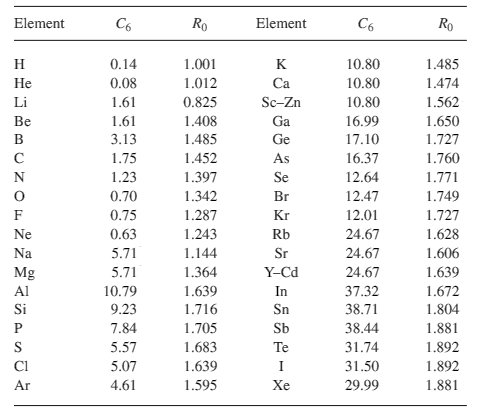
\includegraphics[scale=0.8]{image/C6}
  	\caption[Les paramètres empiriques $C_{6}$ et $R_{0}$ pour DFT-D2]{Les paramètres $C_{6}$ et $R_{0}$} \label{Grimme-parametres}
  \end{figure}
	

	La correction D2 a été employé par Grimme \cite{grimme2006semiempirical} dans systèmes de références comme gaz diatomiques, benzène, anthracène, etc. Les clusters du deuxième groupe du tableau périodique ont donné les plus grands erreurs à cause de la difficile description de systèmes avec cette configuration électronique, laquelle donné des interactions type métalliques.  
	
	Park et al \cite{park2011ab} étudient l'interaction benzène-benzène dans le cas graphite, ils ont trouvé bon corrélation avec les données expérimentales pour les paramètres de maille. 
	
	Plus tard Lee et al \cite{lee2013sum} rapportent les fréquences de vibration des polymorphes de cellulose $I_{\alpha}$ et $I_{\beta}$ dans le logiciel VASP, cependant le valeur du streching OH calculé est 100 cm$^{-1}$ plus petit que l'expérimental. 
	
	
 	\section{DFT-D3}
	
	Les propriétés que présente cette correction par rapport aux versions précédents sont les suivantes :
	\bigskip 
	\begin{itemize}
		\item Elle est moins empirique, les paramètres les plus importants sont calculés par KS-DFT.
		\item L'approche est asympotiquement corrigée pour les fonctionnelles de la densité dans les systèmes limités (molécules) ou systèmes infinites non métalliques.
		\item Elle fournit une description pour les éléments plus relevants (Z=1-94).
		\item Les coefficients de la dispersion des atomes paires et leur cutoff radio sont calculés. 
	\end{itemize}
	\bigskip
	
	L'énergie totale DFT-D3 est donnée par la relation:	
	\begin{equation}
	E_{DFT-D3} = E_{KS-DFT} - E_{disp}
	\end{equation} 
	\bigskip
	
	Où $E_{KS-DFT}$ est l'énergie KS usuel obtenue par la fonctionnelle de la densité choisie, et $E_{disp}$ est la correction à la dispersion qui est représente comme une somme de l'énergie de deux ou trois corps.
	
	\begin{equation}
	E_{disp} = E ^{(2)} + E^{(3)}
	\end{equation}
	
	Le plus important terme de deux corps expression est :
	\begin{equation}
	E^{(2)} = \sum_{AB} \sum_{n=6,8,10...} s_{n}\frac{C_{n}^{AB}}{r^{n}_{AB}} f_{d,n} (r_{AB})
	\end{equation}
	Le premier somme est sur tous les atomes paires du systèmes. $C_{n}^{AB}$ indique la moyenne de nème ordre des coefficients de la dispersion pour les atomes paires AB, et $r_{AB}$ est la distance internucléaire entre eux. Global $s_{n}$ ou facteur d'écaillage est ajusté seulement pour $n>6$ pour assurer l'exactitude asymptotique qui est remplie quand $C_{6}^{AB}$ est exacte. 
	\bigskip
	
	$C_{6}$ terme n'est pas largement écaillage, les plus hauts termes sont nécessaires afin d'adapter le potentiel pour la fonctionnelle de la densité utilisée dans sa région moyenne. Il a été constaté que les termes $n>8$ fassent la méthode légèrement instable dans certains situations, pour cela il a été fait une troncature à $n=8$.
	\bigskip
	
	Pour éviter les singularités dans petits $r_{AB}$ et double comptage des effets de corrélation pour distances intermédiaires, la fonction damping $f_{d,n}$ est employée pour déterminer le range de la correction de la dispersion.
	\bigskip
	
	Il est utilisé une variante proposée par Chai et Head-Gordon\cite{chai2008long} laquelle révèle être numériquement stable et pratique également pour les termes d'ordre supérieur de la dispersion. l'expression de cette fonction est donnée par :
	
	\begin{equation}
	f_{d,n} (r_{AB}) = \frac{1}{1+ 6(r_{AB}/(s_{r,n}R_{0}^{AB}))^{-\alpha_{n}}}
	\end{equation}
	\bigskip
	
	Où $s_{r,n}$ est le facteur d'écaillage dépendant du radio de cutoff $R_{0}^{AB}$. Il remplace $s_{6}$ terme en DFT-D2. 
	\bigskip
	
	Compare au potentiel DFT-D2 le nouveau est moins contraignant pour les petites distances
	mais plus attrayante dans la région typique des interactions de van der waals. Il fournit une séparation plus nette entre le court terme et les effets de dispersion à longue portée.
	
	\subsection{Les coefficients de la dispersion}
	
	
	Au lieu d'utiliser une formule d'interpolation dérivée de manière empirique comme dans DFT-D2, les coefficients de la dispersion sont maintenant calculés par DFT dépendant du temps (TD-DFT), employant des relations de récursion connues pour les termes d'ordre supérieur des multipôles. Le point du départ est la formule de Casimir- Polde\cite{kaplan2006intermolecular} 
	
	\bigskip
	\begin{equation}
	C_{6}^{AB} = \frac{3}{\pi}\int_{0}^{\infty} \alpha^{A} (i\omega) \alpha^{B} (i\omega) d\omega
	\end{equation}
	\bigskip
	
	Où $\alpha(i\omega)$ est la moyenne du dipôle de polarisabilité à la fréquence imaginaire $\omega$. Les coefficients d'ordre supérieur sont calculés récursivement par :
	\bigskip
	\begin{equation}
	C_{8}^{AB} = 3C_{6}^{AB} \sqrt{Q^{A}Q^{B}}
	\end{equation}
	
	et \begin{equation}
	C_{10}^{AB} =\frac{49}{40} \frac{(C_{8}^{AB})^{2}}{C_{6}^{AB}}
	\end{equation}
	
	Avec
	\begin{equation}
	Q^{A} = s_{42}\sqrt{Z^{A}} \frac{\langle r^{4}\rangle r^{A}}{\langle r^{2}\rangle r^{A}}
	\end{equation}
	
	\bigskip
	\subsection{Le terme de Trois Corps}
	\bigskip
	
	La partie à long terme de l'interaction entre trois atomes à l'état fondamental ne correspond pas exactement aux énergies d'interaction prises par paires. Au meilleur de nos connaissances, nous ne sommes pas conscients de toute considération de cet effet dans une structure modèle. Le premier terme non additif de dispersion dérivé du
	la théorie des perturbations de troisième ordre pour trois atomes ABC est :
	
	\begin{equation}
	E^{ABC} = \frac{C_{9}^{ABC}(3\cos\theta_{a}\cos\theta_{b}\cos\theta_{c}+ 1)}{(r_{AB} r_{BC} r_{CA})^{3}}
	\end{equation}
	
	
	Reckien et al \cite{reckien2012implementation} ont mis en place dans le logiciel VASP les corrections D2 et D3. Ils ont étudié métaux, oxydes métalliques, cristaux moléculaires comme benzène, et l'adsorption sur surfaces. Tous les deux méthodes montrent qualitatif et quantitatif resultats des paramètres de maille, cependant la méthode D3 proportionne une meilleure performance.   
	
	\bigskip
	\section{La méthode Tkatchenko-Scheffler (DFT-TS)}
	
	Elle a été propose en 2009 par Tkatchenko et Scheffler\cite{tkatchenko2009accurate}. Nombreux études des structures cristallines ont été menés en utilisant cette correction. Par exemple Kronik et Tkatchenko\cite{kronik2014understanding} étudient le cristal d'Hemozoin d'importance biologique, lequel présent des interactions sur les liaisons hydrogènes. Pour vérifier l'exactitude de la méthode ils sont calculés les paramètres de maille et les modes de vibration du Brushite et le phosphate de calcium hydraté. Bu\u{c}ko et col\cite{buvcko2014extending} ont montre que la méthode peut être utilisée dans systèmes ioniques en changeant le calcul de volume effectif et les charges des atomes par la version itératif de la partition de Hisrfeld.
	
	Dans cette méthode la expression pour l'énergie de dispersion est officiellement identique à la méthode DFT-D2, la plus important différence cependant c'est que les coefficients de dispersion et la fonction damping sont dépendants de la densité de charge. La méthode DFT-TS est capable de prendre en compte les variation à la contribution des interactions de van der waals des atomes dû à leur environnement. 
	
	En effet les coefficient de la dispersion, la polarisabilité et les radios atomiques sont calculés à partir des valeurs des atomes libres selon les expressions suivantes :
	
	\begin{equation}
	\alpha_{i} = \nu_{i} \alpha_{i}^{free}
	\end{equation}
	
	\begin{equation}
	C_{6ii} = \nu_{i}^{2} C_{6ii}^{free}
	\end{equation}
	
	\begin{equation}
	R_{0i} = \left(\frac{\alpha_{i}}{\alpha_{i}^{free}}\right)^{\frac{1}{3}} R_{0i}^{free}
	\end{equation}
	
	Les paramètres $\alpha_{i}^{free}$, $C_{6ii}^{free}$ et $R_{0i}^{free}$ sont tabulé pour tous les éléments des premiers 6 lignes du tableau périodique des éléments, sauf pou les lanthanides. $\nu_{i}$ représente le volume effectif et il est calculé en utilisant la partition de Hirshfeld de la densité des électrons. 
	
	\begin{equation}
	\nu_{i} = \frac{\int r^{3} w_{i}(r)n(r)d^{3}r}{\int n_{i}^{free} (r)d^{3}r}
	\end{equation}
	
	Où n(r) est la densité totale électronique, $n_{i}^{free}$ est la moyenne de la densité électronique sphérique des électrons pour les espèces atomiques neutres libres i. $w_{i}(r)$ est le poids de Hisrfeld et il se définit par les densités atomiques libres.
	
	\begin{equation}
	w_{i}(r)= \frac{n_{i}^{free}(r)}{\sum_{j=1}^{N} n_{j}^{free}(r)}
	\end{equation}
	\bigskip
	
	L'energie de dispersion su système AB est égal : 
	
	\begin{equation}
	E_{dis}= -\frac{1}{2} \sum_{A=1}^{N} \sum_{B=1}^{N} \sum_{L} \frac{C_{6AB}}{R^{6}_{AB,L}} f_{damp}(R_{AB,L})
	\end{equation}
	\bigskip
	
	\subsection{Self-consistent screening dans la méthode Tkatchenko-Scheffler}
	
	Ce variant de la méthode Tkatchenko-Scheffler a été proposé en 2012 par Tkatchenko et col\cite{tkatchenko2012accurate} avec l'objectif d'inclure le dépistage des effets à longe portée des polarisabilités effectifs des atomes. Grâce à l'utilisation de l'équation self-consistent screening d'électrodynamique classique. 
	
	Cela conduit à une description clair de polarisation et dépolarisation pour le tenseur de polarisabilité des molécules et solides. 
	
	Dans cette méthode la fréquence dépendante de la polarisabilité s'obtient la équation self-consistent :
	
	\begin{equation}
	\alpha_{i^{SCS}}(\omega) = \alpha_{i}(\omega) - \alpha_{i}(\omega) \sum_{i\neq j} \tau_{ij} \alpha_{j}^{SCS}(\omega)
	\end{equation} 
	
	où $\tau_{ij}$ est le tenseur d'interaction dipôle- dipôle et $\alpha_{i}(\omega)$ est la fréquence effectif dépendant de la polarisabilité, avec l'expression approximatif : 
	
	\begin{equation}
	\alpha_{i} (\omega) = \frac{\alpha_{i}}{1 + (\omega/\omega_{i})^{2}}
	\end{equation}
	
	avec la fréquence d'excitation moyenne caractéristique $\omega_{i} = \frac{4}{3} \frac{C_{6ii}}{(\alpha_{i})^{2}}$
	\bigskip
	
	Les coefficients de la dispersion sont calcules par l'intégral de Casimir- Polder :
	
	\begin{equation}
	C_{6ii} = \frac{3}{\pi} \int_{0}^{\infty} \alpha_{i}^{SCS} (\omega) \alpha_{i}^{SCS} (\omega) d\omega
	\end{equation}
	
	Les radios atomiques de van der waals sont calcules par renormalisation du radio obtenu par la méthode de Tkatchenko (DFT-TS). 
	
	\begin{equation}
	R_{0i}^{SCS} = \left(\frac{\alpha_{i}^{SCS}}{\alpha_{i}}\right)^{1/3} R_{0i}
	\end{equation}
	
	L'energie de dispersion est évaluée en utilisant la même équation DFT-TS, avec les paramètres corrigés $C_{6ii}^{SCS}$, $\alpha_{i}^{SCS}$ et $R_{0i}^{SCS}$
	
	Cette methode est disponible sur le code VASP grâce à Bu\u{c}ko et col\cite{buvcko2013tkatchenko} qui étudiaient une large gamme de solides comme gaz nobles, cristaux ioniques et moléculaires, structures type chaines et métaux. La méthode conduit à des valeurs raisonnablement précises des propriétés structurelles et de cohésion pour divers types de matières solides. Cependant, l'analyse des résultats a montré que les performances ne sont pas aussi bons pour tous les systèmes et il y a certains types de solides où l'approche échoue définitivement. C'est ainsi que pour les cristaux moléculaires le volume calculé est tout à fait exact, l'énergie de cohésion est exacte pour l'azote, mais surestimée dans une certaine mesure pour les autres systèmes. Ils ont montré que les effets de dépistage sont assez petites pour les systèmes constitués par interactions faibles des atomes neutres et molécules. La méthode est moins performante dans les solides ioniques.
	
	\newpage
	
	\subsection*{Conclusion}
	
	Les interactions faibles ou de Van der Waals jeu un important rôle dans le comportement des systèmes en interaction, en raison de cela la compréhension de ces interactions représentent un domaine d'intérêt surtout dans les calculs théoriques qui ont donné d'importants idées aux scientifiques. 
	\bigskip
	
	Bien qu'il existe de méthodes lesquels prennent en compte la dispersion du systèmes, tels que MP2 ou CCSDT, la taille moléculaire représente une limitant dû au cout de ressources et temps. En conséquence différents approches pour ajouter la dispersion dans les calculs DFT fournissent d'une opportunité pour l'étude de systèmes complexes dont actuellement nous ne connaissons pas vraiment comme ils interagissent. 
	\bigskip
	
	Sans doute chaque système présente caractéristiques spécifiques pour lesquelles une ou autre correction sera plus appropriée, cependant nombreux travaux donnent les pistes à suivre ou les bases pour la démarche dans l'analyse de molécules à l'état solide. 
	\bigskip
	
	En définitive la DFT continue apporter un approche ajusté au molécules de plusieurs atomes dans les différents états d'agrégation. 